\documentclass[tikz,border=5pt]{standalone}
\usepackage{amsmath,amssymb}
\usetikzlibrary{matrix,positioning}
\begin{document}
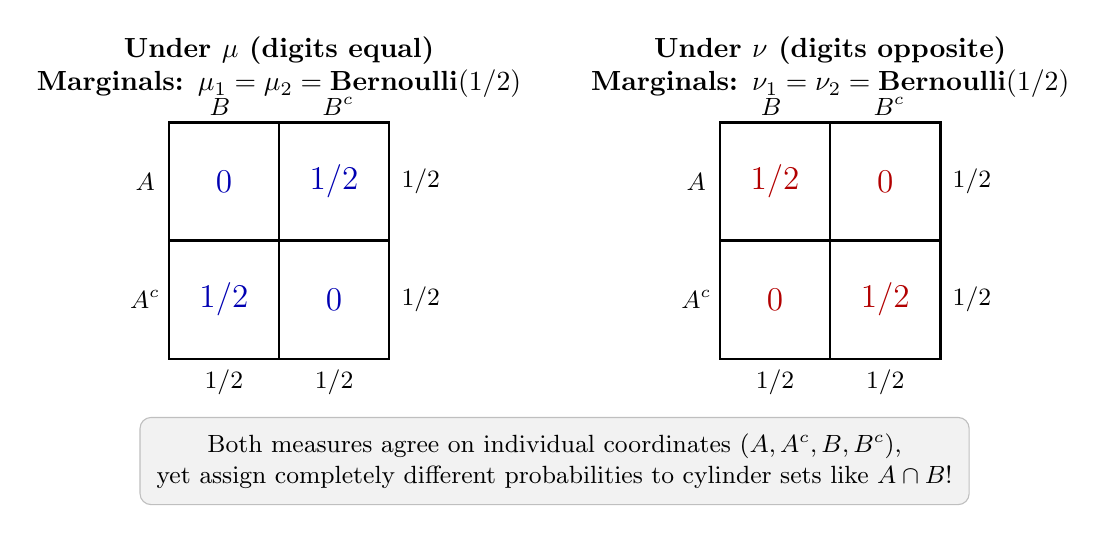
\begin{tikzpicture}[>=latex, font=\small]
  % Table for mu
  \node[font=\bfseries, align=center] at (2, 2.2) {Under $\mu$ (digits equal)\\Marginals: $\mu_1 = \mu_2 = \text{Bernoulli}(1/2)$};
  
  \node at (0.3, 0.75) {$A$};
  \node at (0.3, -0.75) {$A^c$};
  \node at (1.25, 1.7) {$B$};
  \node at (2.75, 1.7) {$B^c$};

  \draw[thick] (0.6, -1.5) rectangle (3.4, 1.5);
  \draw[thick] (2.0, -1.5) -- (2.0, 1.5);
  \draw[thick] (0.6, 0.0) -- (3.4, 0.0);

  \node[font=\large\bfseries, color=blue!70!black] at (1.3, 0.75) {$0$};
  \node[font=\large\bfseries, color=blue!70!black] at (2.7, 0.75) {$1/2$};
  \node[font=\large\bfseries, color=blue!70!black] at (1.3, -0.75) {$1/2$};
  \node[font=\large\bfseries, color=blue!70!black] at (2.7, -0.75) {$0$};

  \node at (3.8, 0.75) {$1/2$};
  \node at (3.8, -0.75) {$1/2$};
  \node at (1.3, -1.8) {$1/2$};
  \node at (2.7, -1.8) {$1/2$};

  % Table for nu
  \begin{scope}[xshift=7cm]
    \node[font=\bfseries, align=center] at (2, 2.2) {Under $\nu$ (digits opposite)\\Marginals: $\nu_1 = \nu_2 = \text{Bernoulli}(1/2)$};
    
    \node at (0.3, 0.75) {$A$};
    \node at (0.3, -0.75) {$A^c$};
    \node at (1.25, 1.7) {$B$};
    \node at (2.75, 1.7) {$B^c$};

    \draw[thick] (0.6, -1.5) rectangle (3.4, 1.5);
    \draw[thick] (2.0, -1.5) -- (2.0, 1.5);
    \draw[thick] (0.6, 0.0) -- (3.4, 0.0);

    \node[font=\large\bfseries, color=red!70!black] at (1.3, 0.75) {$1/2$};
    \node[font=\large\bfseries, color=red!70!black] at (2.7, 0.75) {$0$};
    \node[font=\large\bfseries, color=red!70!black] at (1.3, -0.75) {$0$};
    \node[font=\large\bfseries, color=red!70!black] at (2.7, -0.75) {$1/2$};

    \node at (3.8, 0.75) {$1/2$};
    \node at (3.8, -0.75) {$1/2$};
    \node at (1.3, -1.8) {$1/2$};
    \node at (2.7, -1.8) {$1/2$};
  \end{scope}

  \node[align=center, fill=gray!10, draw=gray!50, rounded corners, inner sep=6pt] at (5.5, -2.8)
    {Both measures agree on individual coordinates ($A, A^c, B, B^c$),\\yet assign completely different probabilities to cylinder sets like $A \cap B$!};
\end{tikzpicture}
\end{document}
